% ============================================================
%   Rapport d'Étude — Intégration des EnR à Mauges Communauté
%   Projet ESIEE Paris x Sopra Steria / Mauges Communauté
% ============================================================
\documentclass[12pt, a4paper]{report}

% ── Encodage & langue ──────────────────────────────────────
\usepackage[utf8]{inputenc}
\usepackage[T1]{fontenc}
\usepackage[french]{babel}

% ── Mise en page ───────────────────────────────────────────
\usepackage[margin=1.5cm]{geometry}
\usepackage{setspace}
\onehalfspacing

% ── Typographie ────────────────────────────────────────────
\usepackage{lmodern}
\usepackage{microtype}
\usepackage{eurosym}

% ── Couleurs & graphiques ──────────────────────────────────
\usepackage[dvipsnames]{xcolor}
\usepackage{graphicx}
\usepackage{float}                % option [H] pour les figures
\usepackage{caption}
\usepackage{subcaption}

% ── Tableaux ───────────────────────────────────────────────
\usepackage{booktabs}
\usepackage{array}
\usepackage{tabularx}
\usepackage{longtable}

% ── Maths ──────────────────────────────────────────────────
\usepackage{amsmath}
\usepackage{amssymb}
\usepackage{siunitx}              % unités physiques : \SI{3.3}{V}
\sisetup{locale = FR}

% ── En-têtes & pieds de page ───────────────────────────────
\usepackage{fancyhdr}
\pagestyle{fancy}
\fancyhf{}

\fancyhead[L]{\small Jusqu’où peut-on augmenter la production EnR locale ?}
\fancyhead[R]{\thepage}
\renewcommand{\headrulewidth}{0.6pt}

% ── Liens hypertexte ───────────────────────────────────────
\usepackage[colorlinks=true, linkcolor=NavyBlue, urlcolor=NavyBlue, citecolor=NavyBlue]{hyperref}

% ── Table des matières ─────────────────────────────────────
\usepackage{tocloft}

% ── Listings (code) ────────────────────────────────────────
\usepackage{listings}
\lstset{
  basicstyle=\ttfamily\scriptsize,
  frame=single,
  breaklines=true,
  inputencoding=utf8,
  extendedchars=true, 
  language=C++
}

% ── Divers ─────────────────────────────────────────────────
\usepackage{enumitem}

% ============================================================
%  MÉTADONNÉES
% ============================================================
\title{
  \vspace{-1cm}
  {\large ESIEE Paris x Sopra Steria}\\[0.5cm]
  {\Huge\bfseries Intégration des EnR à Mauges Communauté}\\[0.3cm]
  {\Large Jusqu'où peut-on augmenter la production EnR locale ?}\\[1.5cm]
  
  % --- Alignement du logo ---
  \centering
  
\includegraphics[width=0.5\linewidth]{images/mauges.jpg}
}

\author{Imran Fagbemi, Noé Quetin, Habib Keita}

\date{\today}

% ============================================================
%  DOCUMENT
% ============================================================
\begin{document}
\maketitle

% ── Résumé ─────────────────────────────────────
\begin{abstract}

Ce document présente les objectifs, contraintes, réflexions et solutions fonctionnelles et énergétiques du projet de simulateur EnR pour Mauges Communauté. Ce dernier répertorie la production et la consommation électrique locale actuelle avant d'établir des trajectoires d'intégration renouvelable supplémentaire guidées par des questionnements territoriaux, techniques et économiques.

Parmi les trois scénarios étudiés (puissance actuelle, +100\% photovoltaïque, +200\% photovoltaïque et +50\% éolien), le scénario C offre le volume annuel produit le plus élevé avec 86,5\% de couverture brute. Toutefois, l'analyse montre que ce scénario entraîne un taux d'écrêtement de 21,0\% qui ne peut pas être résorbé de manière rentable par des batteries centralisées.

La trajectoire optimale recommandée par nos calculs consiste à augmenter le photovoltaïque de +25\% à +50\% et l'éolien de +50\%, tout en mobilisant la flexibilité des usages locaux (recharge méridienne des véhicules électriques et des chauffe-eau). Cette stratégie permet d'atteindre 55,4\% à 65,0\% de couverture réelle avec un taux d'écrêtement inférieur à 3,2\%, tout en respectant les capacités des postes sources du réseau local.

\end{abstract}

% ── Table des matières ─────────────────────────────────────
\tableofcontents
\newpage
% ───────────────────────────────────────────────────────────

% ============================================================
%  CHAPITRE 1 — Contexte actuel et cadre de la démarche
% ============================================================
\chapter*{Contexte actuel et cadre de la démarche}

\section*{Points de départ}

La Communauté d'Agglomération Mauges Communauté (EPCI 200060010), située dans le département de Maine-et-Loire, rassemble 6 communes nouvelles pour une population totale de 123 368 habitants. Ce territoire rural et industrialisé affiche une consommation électrique annuelle mesurée de 802,67 GWh en 2024, soit une moyenne de 5 431 kWh par habitant. La demande électrique est portée par la présence de 369 établissements industriels et par une forte prédominance de maisons individuelles (93,4\% des logements) dont 43,1\% utilisent le chauffage électrique comme mode principal \cite{insee_rp,odre_conso}.

Au 31 décembre 2025, le parc de production renouvelable installé sur le territoire s'élève à 233,51 MW, comprenant 117,73 MWc de photovoltaïque (5 353 installations), 114,40 MW d'éolien terrestre (10 parcs), 1,16 MW de bioénergie et 0,22 MW d'hydraulique. Ce parc assure actuellement un taux de couverture annuel brut de 41,2\% de la consommation locale \cite{odre_registre}.

\section*{Objectifs du cahier des charges}

Le cahier des charges établi par Sopra Steria impose le développement d'un simulateur technico-économique autonome opérant au pas horaire sur cinq années consécutives (2021--2025, soit 43 824 heures). Le simulateur doit évaluer trois scénarios d'installation :
\begin{itemize}
  \item \textbf{Scénario A} : Puissance installée actuelle (117,7 MW PV / 114,4 MW éolien).
  \item \textbf{Scénario B} : +100\% de photovoltaïque (235,5 MW PV / 114,4 MW éolien).
  \item \textbf{Scénario C} : +200\% de photovoltaïque et +50\% d'éolien (353,2 MW PV / 171,6 MW éolien).
\end{itemize}

Les règles de simulation intègrent une perte forfaitaire photovoltaïque de 15\%, la modélisation d'un stockage par batterie d'une capacité équivalente à 2 heures de la puissance PV nominale du scénario avec un rendement aller-retour de 90\%, l'identification des heures de vigilance ($P > 1,2 C$), et le respect d'un seuil réglementaire d'écrêtement annuel maximal de 5\% de la production.

\section*{Formulation des questionnements structurants}

Pour répondre de manière exhaustive aux enjeux du territoire et aux consignes du projet, notre étude s'articule autour de sept questionnements fondamentaux :
\begin{enumerate}
  \item \textbf{Souveraineté et enjeux territoriaux} : Comment l'intégration des EnR résout-elle les problèmes d'indépendance énergétique, de réduction des coûts d'achat réseau, de conformité PCAET et de décarbonation du territoire ?
  \item \textbf{Contribution horaire} : Quelle est la contribution réelle des projets renouvelables à la couverture directe de la consommation locale heure par heure ?
  \item \textbf{Saisonnalité} : Quelle est l'influence de la saisonnalité sur l'équilibre entre production EnR et demande électrique ?
  \item \textbf{Bilan des flux} : Quel est le volume exact des surplus générés et des déficits à combler sur le réseau ?
  \item \textbf{Contraintes réseau} : Quels sont les risques d'injection concentrée et de saturation sur les postes sources HTB/HTA du réseau de distribution Enedis ?
  \item \textbf{Stockage et écrêtement} : Quel est l'intérêt technico-économique réel d'un stockage BESS centralisé comparé à un écrêtement statique ciblé ou à de la flexibilité d'usage ?
  \item \textbf{Trajectoire optimale} : Où situer le seuil d'insertion maximale des EnR et quelle est la trajectoire recommandée pour le territoire ?
\end{enumerate}


% ============================================================
%  CHAPITRE 2 — Résolution des enjeux territoriaux par les EnR
% ============================================================
\chapter{Résolution des enjeux territoriaux par l'intégration des EnR}

\emph{Comment l'intégration des EnR résout-elle les problèmes identifiés de Mauges Communauté (souveraineté, coûts d'achat réseau, objectifs PCAET, décarbonation) ?}

\section{Souveraineté énergétique et réduction des coûts d'achat réseau}

Mauges Communauté dépend historiquement des importations d'électricité sur le réseau national de transport pour couvrir ses 802,67 GWh de consommation annuelle \cite{odre_conso}. Aux tarifs réglementés de vente actuels (environ 0,194~\euro/kWh hors taxes pour le segment résidentiel \cite{cre_trve}), la facture électrique globale du territoire représente plus de 155 millions d'euros par an injectés hors du circuit économique local.

L'augmentation de la production renouvelable locale permet de substituer directement de l'électricité produite sur place à l'électricité achetée sur les marchés de gros. Chaque mégawattheure produit et consommé localement sécurise un coût marginal de production stable sur 20 à 25 ans, prémunissant les ménages, les collectivités et les entreprises contre la volatilité des marchés de l'énergie.

\section{Conformité avec les réglementations et politiques publiques}

Le Plan Climat-Air-Énergie Territorial (PCAET) de Mauges Communauté fixe un objectif de production photovoltaïque de 175 GWh en 2030 et 423 GWh à l'horizon 2050 \cite{pcaet_mauges}. Le scénario A actuel produit 111,8 GWh de photovoltaïque. L'adoption du scénario B porte cette production à 223,6 GWh, permettant au territoire d'atteindre et de dépasser son objectif réglementaire 2030. Cette trajectoire s'inscrit en parfaite cohérence avec le Schéma Régional d'Aménagement, de Développement Durable et d'Égalité des Territoires (SRADDET) des Pays de la Loire.

\section{Réduction de l'empreinte carbone et décarbonation des usages}

Bien que le mix électrique national français présente une faible intensité carbone moyenne (environ 55~g$\text{CO}_2\text{eq}/\text{kWh}$), les heures de pointe hivernales font appel à des moyens de production thermiques fossiles émetteurs de 400 à 1 000~g$\text{CO}_2\text{eq}/\text{kWh}$ \cite{rte_eco2mix}. L'éolien terrestre présent aux Mauges produit préférentiellement en période hivernale et permet d'éviter l'importation d'électricité carbonée lors des pics de consommation.

De plus, la décarbonation à venir du parc automobile (30 600 véhicules électriques projetés en 2035) et le remplacement des 8 794 chaudières au fioul encore présentes dans le territoire par des pompes à chaleur \cite{insee_rp} vont augmenter la demande globale d'électricité d'environ 100 GWh/an. Le développement des EnR locales constitue le levier indispensable pour couvrir ces nouveaux usages sans dégrader le bilan carbone global.

\section{Adéquation entre usages locaux et disponibilité de la production}

Le tissu économique des Mauges comporte une composante agricole importante (8,1\% de la consommation) et un secteur industriel raccordé au réseau HTA/HTB représentant 34,8\% de la demande totale \cite{odre_conso}. Ces activités professionnelles présentent un profil de consommation diurne et régulier en semaine qui coïncide naturellement avec la courbe de production photovoltaïque. Cette concordance structurelle favorise l'autoconsommation collective directe sans nécessiter de report de charge massif.


% ============================================================
%  CHAPITRE 3 — Contribution réelle des EnR et analyse horaire
% ============================================================
\chapter{Contribution réelle des EnR et profil de consommation heure par heure}

\emph{Quelle est la contribution réelle des projets renouvelables à la consommation locale heure par heure ?}

\section{Méthodologie de reconstruction des courbes de charge}

En l'absence de courbes de charge individuelles publiées à l'échelle communale pour des raisons de secret statistique, la courbe de consommation horaire du territoire a été reconstruite en combinant le volume annuel mesuré sur le territoire \cite{odre_conso} avec les profils sectoriels régionaux d'Enedis (Méthode S sur 2024--2025 \cite{enedis_profils}) et les profils globaux d'Eco2Mix (Méthode R sur 2021--2023 \cite{rte_eco2mix}).

L'analyse approfondie des données ODRÉ a révélé qu'une part de 16,2\% de la consommation industrielle du territoire (130,2 GWh/an) est raccordée directement au réseau de transport RTE. Cette consommation industrielle haute tension a été modélisée par un profil plat à puissance constante, reflétant le fonctionnement continu des procédés industriels locaux.

\section{Calibrage des facteurs de charge locaux}

Les facteurs de charge régionaux issus d'Eco2Mix ont été ajustés aux performances réelles des installations du territoire enregistrées au registre national \cite{odre_registre}. Les facteurs de charge moyens locaux retenus s'élèvent à 12,1\% pour le photovoltaïque (soit un productible de 1 060 kWh/kWc) et 22,4\% pour l'éolien terrestre.

Un traitement spécifique a permis de corriger le biais introduit dans les séries régionales à partir de la fin de l'année 2022 par la mise en service du parc éolien en mer de Saint-Nazaire, garantissant que les profils appliqués aux Mauges reflètent exclusivement la productivité de l'éolien terrestre.

\section{Contribution horaire au bilan local (Scénario A)}

Au pas horaire, la puissance moyenne appelée par le territoire s'établit à 91,6 MW, avec une pointe hivernale mesurée à 163,6 MW (le 10 janvier 2024 à 10h00 UTC \cite{meteo_france}). La figure \ref{fig:semaine_type} illustre le comportement horaire du système lors d'une semaine type d'hiver et d'été.

\begin{figure}[H]
  \centering
  \begin{subfigure}[b]{\textwidth}
    \centering
    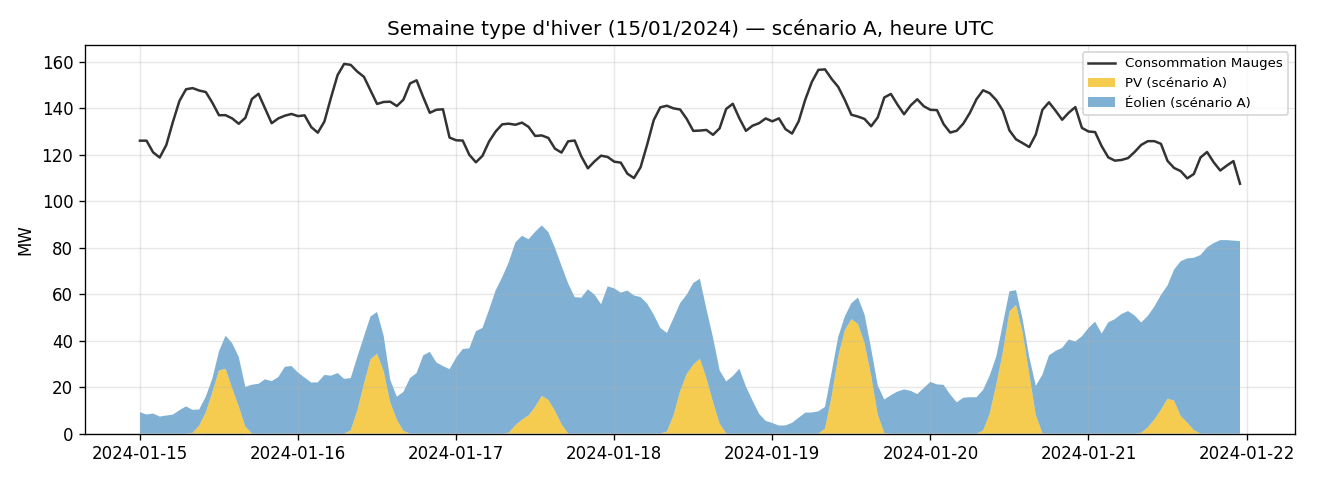
\includegraphics[width=\textwidth]{images/01_semaine_hiver.png}
    \caption{Semaine d'hiver (janvier)}
  \end{subfigure}
  \hfill
  \begin{subfigure}[b]{\textwidth}
    \centering
    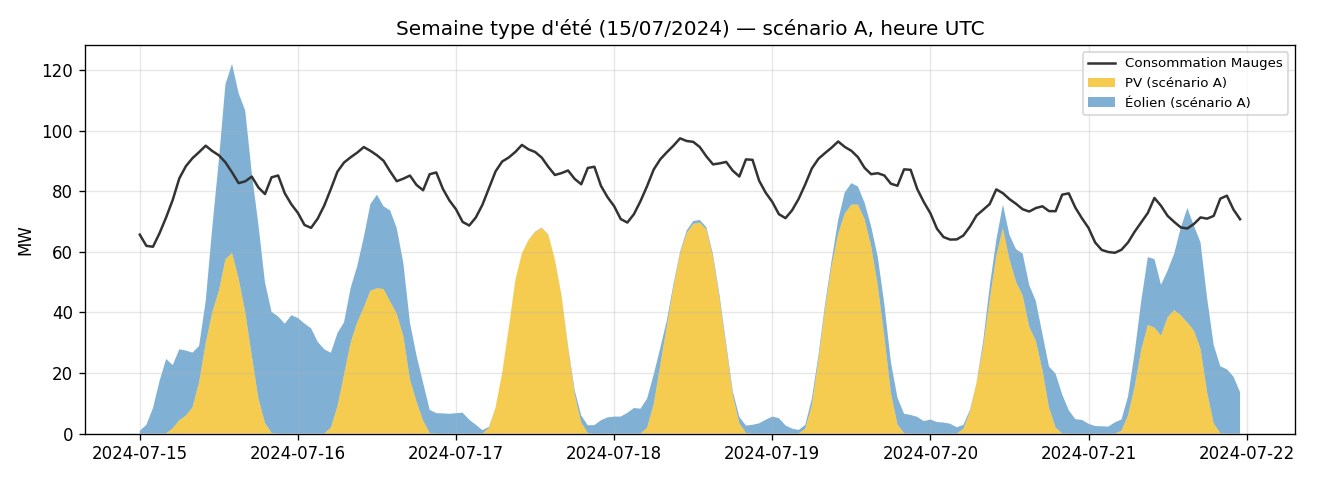
\includegraphics[width=\textwidth]{images/02_semaine_ete.png}
    \caption{Semaine d'été (juillet)}
  \end{subfigure}
  \caption{Équilibre horaire entre consommation et production EnR (Scénario A, année 2024).}
  \label{fig:semaine_type}
\end{figure}

En scénario A, la production EnR couvre instantanément la totalité de la consommation locale pendant 1 240 heures par an. Le taux d'autonomie horaire réel (part de la consommation couverte directement sans stockage) atteint 41,6\% sur la moyenne des cinq années simulées.


% ============================================================
%  CHAPITRE 4 — Saisonnalité, surplus et déficits énergétiques
% ============================================================
\chapter{Saisonnalité, surplus et déficits énergétiques}

\emph{Quelle est l'influence de la saisonnalité sur l'équilibre entre production et consommation, et quel est le volume exact des surplus et déficits ?}

\section{Influence de la saisonnalité sur l'équilibre électrique}

L'équilibre entre la production renouvelable et la consommation présente une opposition saisonnière marquée :
\begin{itemize}
  \item En hiver (novembre à février), la consommation atteint son maximum sous l'effet du chauffage électrique des 93,4\% de maisons individuelles \cite{insee_rp}. Durant cette période, la production photovoltaïque est à son niveau le plus bas (facteur de charge de 4 à 6\%), tandis que l'éolien terrestre atteint son optimum (facteur de charge de 33,7\%).
  \item En été (mai à août), la consommation diminue de 30\% en raison de l'arrêt du chauffage, tandis que la production photovoltaïque atteint son pic.
\end{itemize}

Cette complémentarité fait de l'éolien terrestre un vecteur clé de l'équilibre hivernal du territoire.

\section{Quantification des surplus et des déficits}

L'évaluation menée sur les 43 824 heures de la période 2021--2025 permet de quantifier précisément les flux d'énergie pour chaque scénario. Le tableau \ref{tab:bilan_surplus_deficits} rassemble les résultats moyens obtenus.

\begin{table}[H]
\centering
\caption{Bilan annuel des flux d'énergie (moyennes 2021--2025).}
\label{tab:bilan_surplus_deficits}
\begin{tabularx}{\textwidth}{lXXX}
\toprule
Grandeur énergétique & Scénario A & Scénario B & Scénario C \\
\midrule
Consommation annuelle ($C$) & 802,7 GWh & 802,7 GWh & 802,7 GWh \\
Production EnR totale ($P$) & 343,7 GWh & 467,5 GWh & 700,7 GWh \\
Énergie couverte simultanément & 334,0 GWh & 397,3 GWh & 495,2 GWh \\
Déficit à importer du réseau & 468,7 GWh & 405,4 GWh & 307,5 GWh \\
Surplus total ($P > C$) & 6,7 GWh & 66,5 GWh & 193,9 GWh \\
Écrêtement critique ($P > 1,2 C$) & 2,1 GWh & 42,1 GWh & 148,9 GWh \\
\bottomrule
\end{tabularx}
\end{table}

\section{Analyse des heures de vigilance réseau}

Le cahier des charges définit une heure de vigilance lorsque la production locale dépasse 120\% de la consommation horaire. En scénario A, cette situation se produit seulement 175 heures par an. En scénario B (+100\% PV), le nombre d'heures de vigilance s'élève à 1 240 heures/an. En scénario C, le réseau entre en vigilance durant 2 271 heures/an, soit plus de 25\% de l'année.


% ============================================================
%  CHAPITRE 5 — Risques d'injection concentrée et postes sources
% ============================================================
\chapter{Risques d'injection concentrée et contraintes des postes sources}

\emph{Quels sont les risques d'injection concentrée sur les postes sources du réseau de distribution ?}

\section{Répartition géographique des capacités de production}

L'analyse de la base de données des installations raccordées \cite{odre_registre} montre une répartition très hétérogène du parc EnR entre les six communes de Mauges Communauté :
\begin{itemize}
  \item Chemillé-en-Anjou regroupe 92,1 MW (dont 63,2 MW éoliens et 28,9 MW PV), soit 39,4\% de la puissance totale du territoire.
  \item Montrevault-sur-Èvre accueille 38,3 MW (principalement éoliens).
  \item Beaupréau-en-Mauges dispose de 21,0 MW.
  \item Sèvremoine, Mauges-sur-Loire et Orée d'Anjou se partagent le solde.
\end{itemize}

\section{Capacité d'accueil des postes sources du réseau}

Le territoire des Mauges est desservi par quatre postes sources HTB/HTA principaux implantés sur le périmètre communal (Chemillé CHEMI, St-Pierre-Montlimart SSMO5, Le Genêt GENET et La Sourdrie SOURD), complétés par six postes périphériques \cite{capareseau}.

Les capacités d'accueil réservées au titre du Schéma Régional de Raccordement au Réseau des Énergies Renouvelables (S3REnR) ont été collectées via Caparéseau \cite{capareseau} et comparées aux puissances d'injection de pointe générées par les scénarios (tableau \ref{tab:postes_sources}).

\begin{table}[H]
\centering
\caption{Analyse des contraintes de puissance sur les postes sources principaux (en MW).}
\label{tab:postes_sources}
\begin{tabularx}{\textwidth}{lXXXXX}
\toprule
Poste Source & Parc A actuel & Ajout Scénario B & Ajout Scénario C & Capacité réservée S3REnR & Marge disponible \\
\midrule
CHEMI (Chemillé) & 85,2 & +22,4 & +76,1 & 60,0 & 23,1 \\
SSMO5 (St-Pierre) & 38,3 & +22,3 & +52,5 & 24,5 & 0,9 \\
GENET (Beaupréau) & 21,0 & +6,6 & +20,4 & 7,5 & 0,5 \\
RECOU (Recouvrance) & 18,7 & +18,7 & +37,3 & 54,0 & 33,3 \\
\bottomrule
\end{tabularx}
\end{table}

\section{Analyse des dépassements de capacité}

Dès le scénario B, le poste source de St-Pierre-Montlimart (SSMO5) subit un dépassement de sa capacité réservée de 21,4 MW, et le poste du Genêt de 6,1 MW. En scénario C, le poste de Chemillé (CHEMI) dépasse sa marge disponible de 53,0 MW.

Sans travaux de renforcement du réseau HTA ou transfert de capacité entre postes, le scénario C provoquerait des saturations thermiques et des surtensions répétées, entraînant la déconnexion de sécurité des onduleurs photovoltaïques.


% ============================================================
%  CHAPITRE 6 — Éléments technico-économiques du stockage BESS
% ============================================================
\chapter{Évaluation technico-économique du stockage BESS et de l'écrêtement}

\emph{Quel est l'intérêt technico-économique réel d'un stockage par batterie ou d'un écrêtement ciblé ?}

\section{Algorithmes de pilotage de la batterie}

Deux stratégies de pilotage du stockage par batterie ont été développées et comparées :
\begin{enumerate}
  \item \textbf{Pilotage glouton} : La batterie charge dès que la production locale dépasse la consommation ($P > C$) et se décharge dès qu'un déficit apparaît ($P < C$).
  \item \textbf{Pilotage ciblé (Peak Shaving)} : La batterie ne déclenche sa charge que lorsque la production franchit le seuil de vigilance ($P > 1,2 C$).
\end{enumerate}

En scénario C, l'algorithme glouton remplit la batterie dès les premières heures de la matinée. Lorsque survient la pointe solaire de mi-journée (13h--14h), la batterie est déjà saturée ($\text{SOC} = 100\%$). Le pilotage ciblé préserve la capacité du stockage pour raboter le sommet de la courbe d’injection, réduisant l'écrêtement de 8,40\% à 6,32\%.

\section{Évaluation financière de la solution batterie}

L'analyse économique s'appuie sur le jeu de données officiel NREL 2025 \cite{nrel_storage} : un coût d'investissement (CAPEX) de 395~\euro/kWh installé pour un système lithium-ion de 2 heures, des coûts d'exploitation (OPEX) de 49~\euro/kW/an, une durée de vie de 15 ans et un taux d'actualisation de 4\%. Les résultats d'actualisation financière sont synthétisés dans le tableau \ref{tab:van_batterie}.

\begin{table}[H]
\centering
\caption{Bilan économique du stockage centralisé par batterie (durée 15 ans).}
\label{tab:van_batterie}
\begin{tabularx}{\textwidth}{lXXXX}
\toprule
Scénario & Capacité BESS & Investissement CAPEX & Gain annuel d'autoconsommation & Valeur Actuelle Nette (VAN) \\
\midrule
Scénario B (Glouton) & 471 MWh & 186 M\euro & +9,7 M\euro/an & $-161$ M\euro \\
Scénario B (Ciblé) & 471 MWh & 186 M\euro & +6,4 M\euro/an & $-197$ M\euro \\
Scénario C (Glouton) & 706 MWh & 279 M\euro & +20,7 M\euro/an & $-173$ M\euro \\
Scénario C (Ciblé) & 706 MWh & 279 M\euro & +17,9 M\euro/an & $-204$ M\euro \\
\bottomrule
\end{tabularx}
\end{table}

Les coûts de maintenance annuels de la batterie absorbant une part majeure des gains générés par l'électricité évitée, la Valeur Actuelle Nette est fortement négative dans tous les cas de figure. La batterie centralisée n'est pas une solution économiquement rentable.

\section{Écrêtement statique sans stockage}

Si l'on renonce à la batterie, le scénario B présente un taux d'écrêtement de 8,20\% au-dessus du seuil de vigilance. Pour ramener cet écrêtement sous la limite réglementaire de 5\%, il suffit de dissiper ou de brider 3,20\% de la production annuelle, soit 15,0 GWh/an. Valorisé au prix de marché du surplus (20~\euro/MWh \cite{cre_trve}), ce bridage représente un coût annuel de seulement 300 000~\euro/an, à comparer aux 186 M\euro{} d'investissement nécessaires pour la batterie.


% ============================================================
%  CHAPITRE 7 — Seuil d'insertion maximale et trajectoire
% ============================================================
\chapter{Seuil d'insertion maximale et trajectoire recommandée}

\emph{Où situer le seuil d'insertion maximale des EnR et quelle est la trajectoire optimale recommandée ?}

\section{Gisements fonciers et potentiel solaire du territoire}

L'analyse des bases de données cadastrales du Cerema et de l'IGN \cite{cerema_pv} montre que Mauges Communauté dispose d'un potentiel photovoltaïque brut en toiture de 2 750 MWc (2 900 GWh/an).

Le PCAET territorial vise la mobilisation de 15\% des toitures (soit 413 MWc / 438 GWh/an \cite{pcaet_mauges}). De plus, l'inventaire des parkings de plus de 500~$\text{m}^2$ révèle une surface de 95 hectares \cite{cerema_pv}, permettant d'installer 63 MWc d'ombrières en application de la loi APER. La contrainte foncière n'est donc pas le facteur limitant.

\section{Acceptabilité sociale et dynamique de la mobilité électrique}

L'acceptabilité de l'éolien terrestre atteint un seuil de saturation locale en raison de la densité de parcs existants dans le nord du territoire (10 parcs, 114,4 MW). La concertation sur les Zones d'Accélération des Énergies Renouvelables (ZAER) montre une préférence des riverains pour le développement du solaire sur toitures industrielles et agricoles.

Sur le volet de la mobilité, le territoire compte 3 000 véhicules électriques rechargeables fin 2025 (soit 24,3 VE pour 1 000 habitants) \cite{ore_voitures}. Les projections à l'horizon 2035 prévoient un parc de 30 600 véhicules électriques \cite{insee_rp}.

\section{Potentiel de flexibilité de la demande locale}

La modélisation de l'électrification des usages à l'horizon 2035 met en évidence une capacité d'absorption considérable :
\begin{itemize}
  \item Le pilotage de la recharge de 15 000 véhicules électriques durant la pause méridienne (10h--16h) offre une puissance d'absorption modulable de 50 à 100 MW.
  \item Le déplacement de la chauffe des 26 000 ballons d'eau chaude sanitaires résidentiels de la nuit vers la mi-journée permet d'absorber 29 MW supplémentaires de puissance solaire.
\end{itemize}

\section{Recommandation de la trajectoire optimale}

Au terme de l'évaluation technico-économique, la trajectoire recommandée pour Mauges Communauté (baptisée « Mix Optimal Mauges ») consiste à :
\begin{enumerate}
  \item Limiter le développement photovoltaïque à une hausse de +25\% à +50\% (soit 147 à 176 MWc au total) en ciblant en priorité les toitures des bâtiments agricoles/industriels et les ombrières de parking.
  \item Accroître le parc éolien terrestre de +50\% (soit 171,6 MW au total) en orientant les nouveaux mats vers les zones identifiées au PCAET disposant de capacité réseau sur le poste de Recouvrance.
  \item Instaurer un pilotage tarifaire méridien pour la recharge des véhicules électriques et des chauffe-eau sanitaires.
\end{enumerate}

Cette trajectoire permet d'atteindre un taux de couverture réelle de 55,4\% à 65,0\% avec un taux d'écrêtement contenu à 3,2\%, garantissant l'équilibre du réseau local sans aucun surcoût d'investissement en stockage par batterie.


% ============================================================
%  BIBLIOGRAPHIE
% ============================================================
\begin{thebibliography}{99}

\bibitem{insee_rp}
INSEE, \textit{Dossier complet -- CA Mauges Communauté (EPCI 200060010)}, Recensement de la population 2023, Institut National de la Statistique et des Études Économiques, 2026. \url{https://www.insee.fr/fr/statistiques/2011101?geo=EPCI-200060010}

\bibitem{odre_conso}
ODRÉ, \textit{Consommation d'électricité et de gaz par EPCI}, Données 2012--2024, Open Data Réseaux Énergies, 2025. \url{https://odre.opendatasoft.com/explore/dataset/conso-epci-annuelle/}

\bibitem{odre_registre}
ODRÉ, \textit{Registre national des installations de production et de stockage d'électricité}, Données au 31/12/2025, Open Data Réseaux Énergies, 2026. \url{https://odre.opendatasoft.com/explore/dataset/registre-national-installation-production-stockage-electricite-agrege-311225/}

\bibitem{rte_eco2mix}
RTE, \textit{Données régionales éCO2mix consolidées (Pays de la Loire)}, Données 2021--2025, Réseau de Transport d'Électricité. \url{https://odre.opendatasoft.com/explore/dataset/eco2mix-regional-cons-def/}

\bibitem{enedis_profils}
Enedis, \textit{Profils de consommation et d'injection par segment de puissance}, Plateforme Data-Fair Enedis, 2024--2025. \url{https://opendata.enedis.fr/datasets/conso-inf36-region}

\bibitem{meteo_france}
Météo-France, \textit{Données climatologiques de base horaires (Stations de Saint-Florent-le-Vieil n°49276001 et Beaucouzé n°49020001)}, 2021--2025. \url{https://www.data.gouv.fr/fr/datasets/donnees-climatologiques-de-base-horaires/}

\bibitem{pcaet_mauges}
Mauges Communauté, \textit{Plan Climat-Air-Énergie Territorial (PCAET) -- Rapport de présentation et objectifs 2030-2050}, 2020. \url{https://www.maugescommunaute.fr/}

\bibitem{cre_trve}
CRE, \textit{Délibération relative aux Tarifs Réglementés de Vente d'Électricité (TRVE)}, Commission de Régulation de l'Énergie, 2026. \url{https://www.cre.fr/}

\bibitem{capareseau}
Enedis et RTE, \textit{Caparéseau -- Capacités d'accueil des réseaux électriques pour l'injection d'énergies renouvelables}, Données des postes sources 2026. \url{https://www.capareseau.fr/}

\bibitem{nrel_storage}
NREL, \textit{Cost Projections for Utility-Scale Battery Storage: 2025 Update}, National Renewable Energy Laboratory, 2025. \url{https://www.nrel.gov/docs/fy25osti/89000.pdf}

\bibitem{cerema_pv}
Cerema et IGN, \textit{Potentiel solaire photovoltaïque des toitures et des parkings d'après la BD TOPO}, Données 2023. \url{https://www.cerema.fr/}

\bibitem{ore_voitures}
Agence ORE, \textit{Voitures particulières immatriculées par commune et EPCI}, Open Data Réseaux Énergies, 2025. \url{https://www.agenceore.fr/}

\end{thebibliography}

\end{document}
